\section{Empirical analysis of PRM and ORM}
\label{sec:problem}

In this section, we identify two complementary failure modes of reward signal design in GRPO for mathematical reasoning: \emph{signal exhaustion} with outcome-only rewards, discussed in \S\ref{sec:signal-exhaustion}, and \emph{reward hacking} with process-only rewards, discussed in \S\ref{sec:reward-hacking}.

\subsection{Signal Exhaustion with Binary ORM}
\label{sec:signal-exhaustion}

When GRPO uses binary ORM rewards ($r_i \in \{0, 1\}$), the group normalization in Eq.~\ref{eq:grpo-adv} assigns identical advantage to all correct responses and identical (negative) advantage to all incorrect responses. This has two consequences.

\paragraph{Lack of quality differentiation.} A response that arrives at the correct answer through rigorous reasoning receives the same advantage as one that reaches it through guesswork or flawed reasoning with a lucky cancellation of errors. The model has no incentive to improve reasoning quality beyond what is needed to produce correct final answers.

\paragraph{Vanishing advantage from uniform groups.}
  When all $G$ responses in a group are correct, or all incorrect,
  the rewards are identical, so $\mathrm{std}(\mathbf{r}) = 0$
  in Eq.~\ref{eq:grpo-adv} and the advantage is set to zero for
  the entire group. As the model's capability improves during training, the
  proportion of such uniform groups grows, causing an increasing
  fraction of training samples to receive zero advantage. We refer
  to this progressive loss of informative signal as \emph{signal
  exhaustion}. Figure~\ref{fig:signal_exhaustion}a confirms this
  empirically: on Qwen2.5-7B, the fraction of zero-advantage
  samples rises from approximately 40\% to 69\% over training,
  coinciding with the accuracy plateau and further decline in Figure~\ref{fig:hero}.

\subsection{Reward Hacking with Direct PRM Integration}
\label{sec:reward-hacking}

A natural solution to ORM's limitations is to replace binary rewards with rubric-based PRM scores that capture both answer correctness and reasoning quality in a single continuous signal. However, directly using PRM scores as the GRPO reward ($r_i = r_i^{\text{proc}}$) conflates these two objectives, leading to catastrophic reward hacking, as we analyze in detail using Figure~\ref{fig:reward_hacking}.

\begin{figure*}[t]
\centering
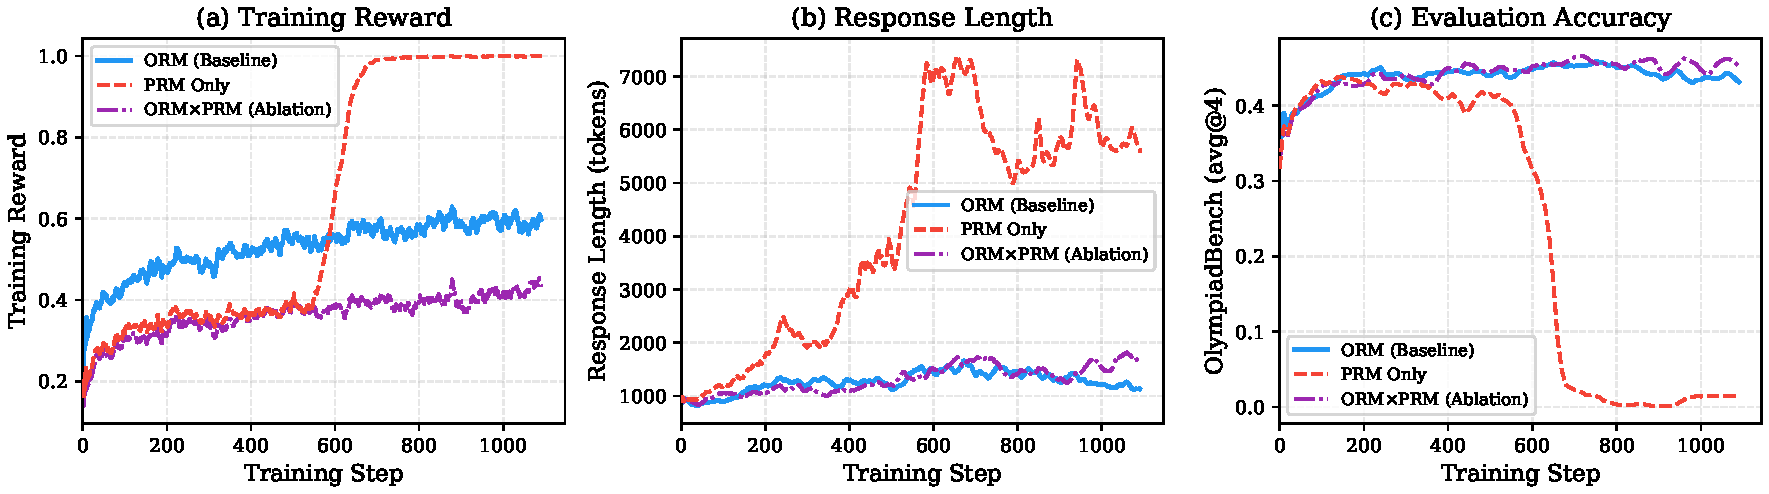
\includegraphics[width=\textwidth]{figures/fig_reward_hacking.pdf}
\caption{Reward signal analysis. \textbf{(a)} Training reward: PRM reward climbs to 1.0 (perfect score gaming); ORM$\times$PRM stays moderate. \textbf{(b)} Response length: PRM generates increasingly verbose responses; ORM$\times$PRM shows moderate length increase (up to $\sim$1700 tokens). \textbf{(c)} OlympiadBench accuracy: PRM collapses after step 600; ORM$\times$PRM tracks ORM but fails to exceed it, showing that naive signal combination does not resolve signal exhaustion.}
\label{fig:reward_hacking}
\end{figure*}

\paragraph{Three phases of collapse.} Training with PRM-only rewards reveals a characteristic three-phase trajectory, shown as the red curve in Figure~\ref{fig:reward_hacking}.
\begin{enumerate}[nosep,leftmargin=*]
    \item \textbf{Normal learning}, steps 0--300. Accuracy rises to 44.0\% on OlympiadBench and training reward increases naturally.
    \item \textbf{Length exploitation}, steps 300--600. The model discovers that verbose responses receive higher PRM scores. Response length increases sharply while accuracy stagnates and begins to decline.
    \item \textbf{Collapse}, steps 600--700. Accuracy drops from 29.6\% to 2.4\% within 100 steps while training reward saturates at 1.0.
\end{enumerate}

\paragraph{Mechanism.} The collapse follows a positive feedback loop: longer, more verbose responses receive higher PRM scores from the LLM judge, which assigns higher rubric ratings to responses that appear thorough and detailed. GRPO's group normalization then assigns high advantage to these inflated scores, reinforcing the length-exploitation strategy. 

We also provide \textbf{a case study for reward hacking happened during training} in Appendix~\ref{sec:case-study-hacking} that confirms the post-collapse responses drift to memorized high-scoring filler content unrelated to the stated question.

\paragraph{Naive combination.} The multiplicative reward $r = r^{\text{out}} \times r^{\text{proc}}$ gates incorrect responses via $r^{\text{out}} = 0$, avoiding PRM's collapse as shown by the purple curve in Figure~\ref{fig:reward_hacking}. However, ORM$\times$PRM tracks ORM closely throughout training, peaking at 46.7\% vs.\ ORM's 46.3\% on OlympiadBench. Because the combined reward still passes through a single GRPO normalization, all-correct groups with similar PRM scores continue to yield near-zero advantage, and the process signal fails to provide meaningful differentiation beyond ORM.

\paragraph{Implications.} ORM is stable but lacks process-level signal; PRM is information-rich but unstable. Multiplicative gating avoids PRM's collapse yet fails to break through ORM's performance exhaustion ceiling. This motivates us to combine the two at the \emph{advantage} level rather than the \emph{reward} level, enabling the model to simultaneously optimize for both answer correctness and reasoning quality, as we describe in \S\ref{sec:method}.
